\documentclass[a4paper,12pt,oneside,final,spanish]{article}
%titlepage: pone el título en una página aparte
%twocolumn
\usepackage{babel} %Para el lenguaje [spanish]
\usepackage[utf8]{inputenc} %Para reconocer todos los símbolos
\usepackage[T1]{fontenc}
\usepackage{textcomp}
\usepackage{amsmath}
\usepackage{amsfonts}
\usepackage{amssymb}
\usepackage[margin=1.5cm]{geometry} %Márgenes
\usepackage[T1]{fontenc}
\usepackage{graphicx}
\usepackage{enumerate}
\usepackage{hyperref}
%\pagestyle{headings}

\title{\Huge Tecnologías para la Web Semántica\\
Trabajo Práctico Nº4\\
Ontologías}
\author{Darién Julián Ramírez}
\date{\vspace{-5ex}}

\begin{document}

\maketitle %Crea la página de título

\section*{Ejercicio 1}

Seleccione seis ontologías pertenecientes a diferentes categorías. Elabore un informe conteniendo los siguientes datos:
\begin{quote}
\begin{enumerate}[a.]
\item Nombre – URL.
\item Grupo u organismo de desarrollo.
\item Categoría. En caso de ser de dominio, especifique de qué dominio se trata. \item Justifique.
\item Descripción.
\item Cantidad de términos (aprox.).
\item Taxonomía (jerarquía de componentes) o modelo.
\end{enumerate}
\end{quote}

\dotfill

\begin{quote}
Time Ontology in OWL - https://www.w3.org/TR/2016/WD-owl-time-20160712\\
W3C\\
Ontología general\\
La ontología OWL-Time es una ontología OWL-2 DL [owl2-direct-semantics] de conceptos temporales, para describir las propiedades temporales de los recursos en el mundo o descritas en páginas web. La ontología proporciona un vocabulario para expresar hechos sobre relaciones topológicas entre instantes e intervalos, junto con información sobre duraciones y sobre la posición temporal incluyendo la información de fecha y hora.\\

MarineTLO ontology - http://www.ics.forth.gr/isl/MarineTLO/\\
W3C\\
Ontología de dominio. Dominio marino también aplicable al dominio terrestre.\\
MarineTLO es una ontología de alto nivel para el dominio marino (también aplicable al dominio terrestre). Abordar la necesidad de contar con conjuntos integrados de datos sobre especies marinas y, por lo tanto, ayudar a la investigación sobre especies y biodiversidad.
Proporciona un modelo de núcleo unificado y coherente para la asignación de esquemas que permite formular y responder consultas que no pueden ser respondidas por ninguna fuente individual.\\

Ontología Gestión de Recursos Humanos - http://mayor2.dia.fi.upm.es/oeg-upm/index.php/es/ontologies/99hrmontology/index.html\\
Boris Villazón-Terrazas, Jaime Ramírez y Asunción Gómez-Pérez\\
Ontología de dominio. Esta ontología actuará como un lenguaje común mediante un conjunto de vocabularios controlados para describir los detalles de una oferta de trabajo y el curriculum vitae del demandante de empleo.\\
Está compuesta por trece ontologías contando con 3206 conceptos, 277 atributos, 1428 instancias y 1592 axiomas.

\begin{center}
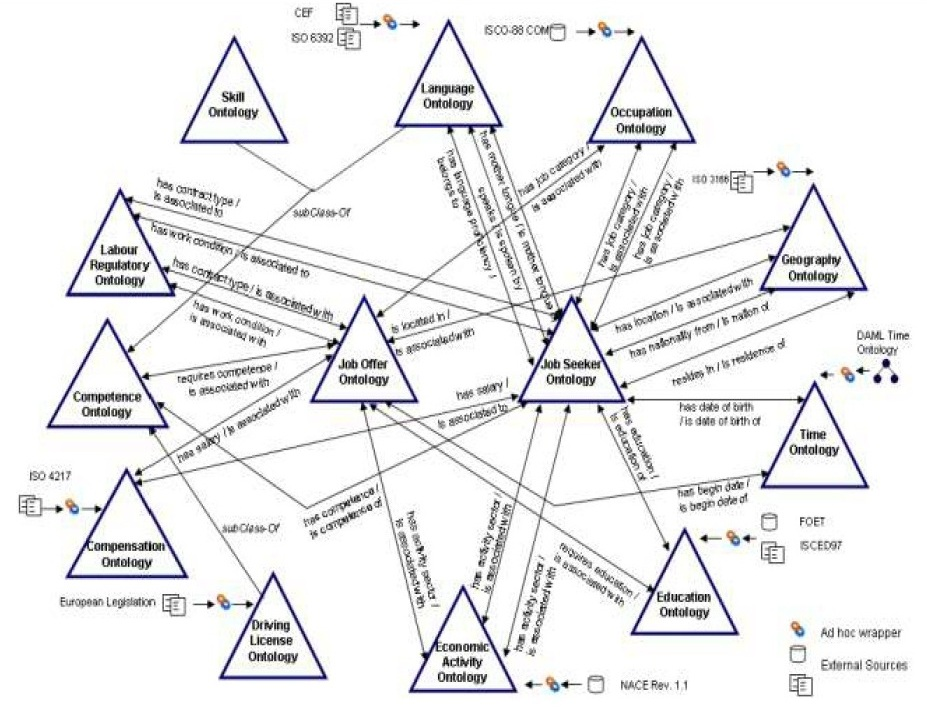
\includegraphics[width=0.9\linewidth,keepaspectratio]{ont1.jpg}
\end{center}

Web semántica - http://bvs.sld.cu/revistas/aci/aci030605.htm\\
Lic. Keilyn Rodríguez Perojo y Lic. Rodrigo Ronda León\\
Ontología de dominio. Un nuevo enfoque para la organización y recuperación de información en el web. Especifica  la  estructura  general  de  la  web  semántica  y  sus principales componentes. Contiene 21 términos.

\begin{center}
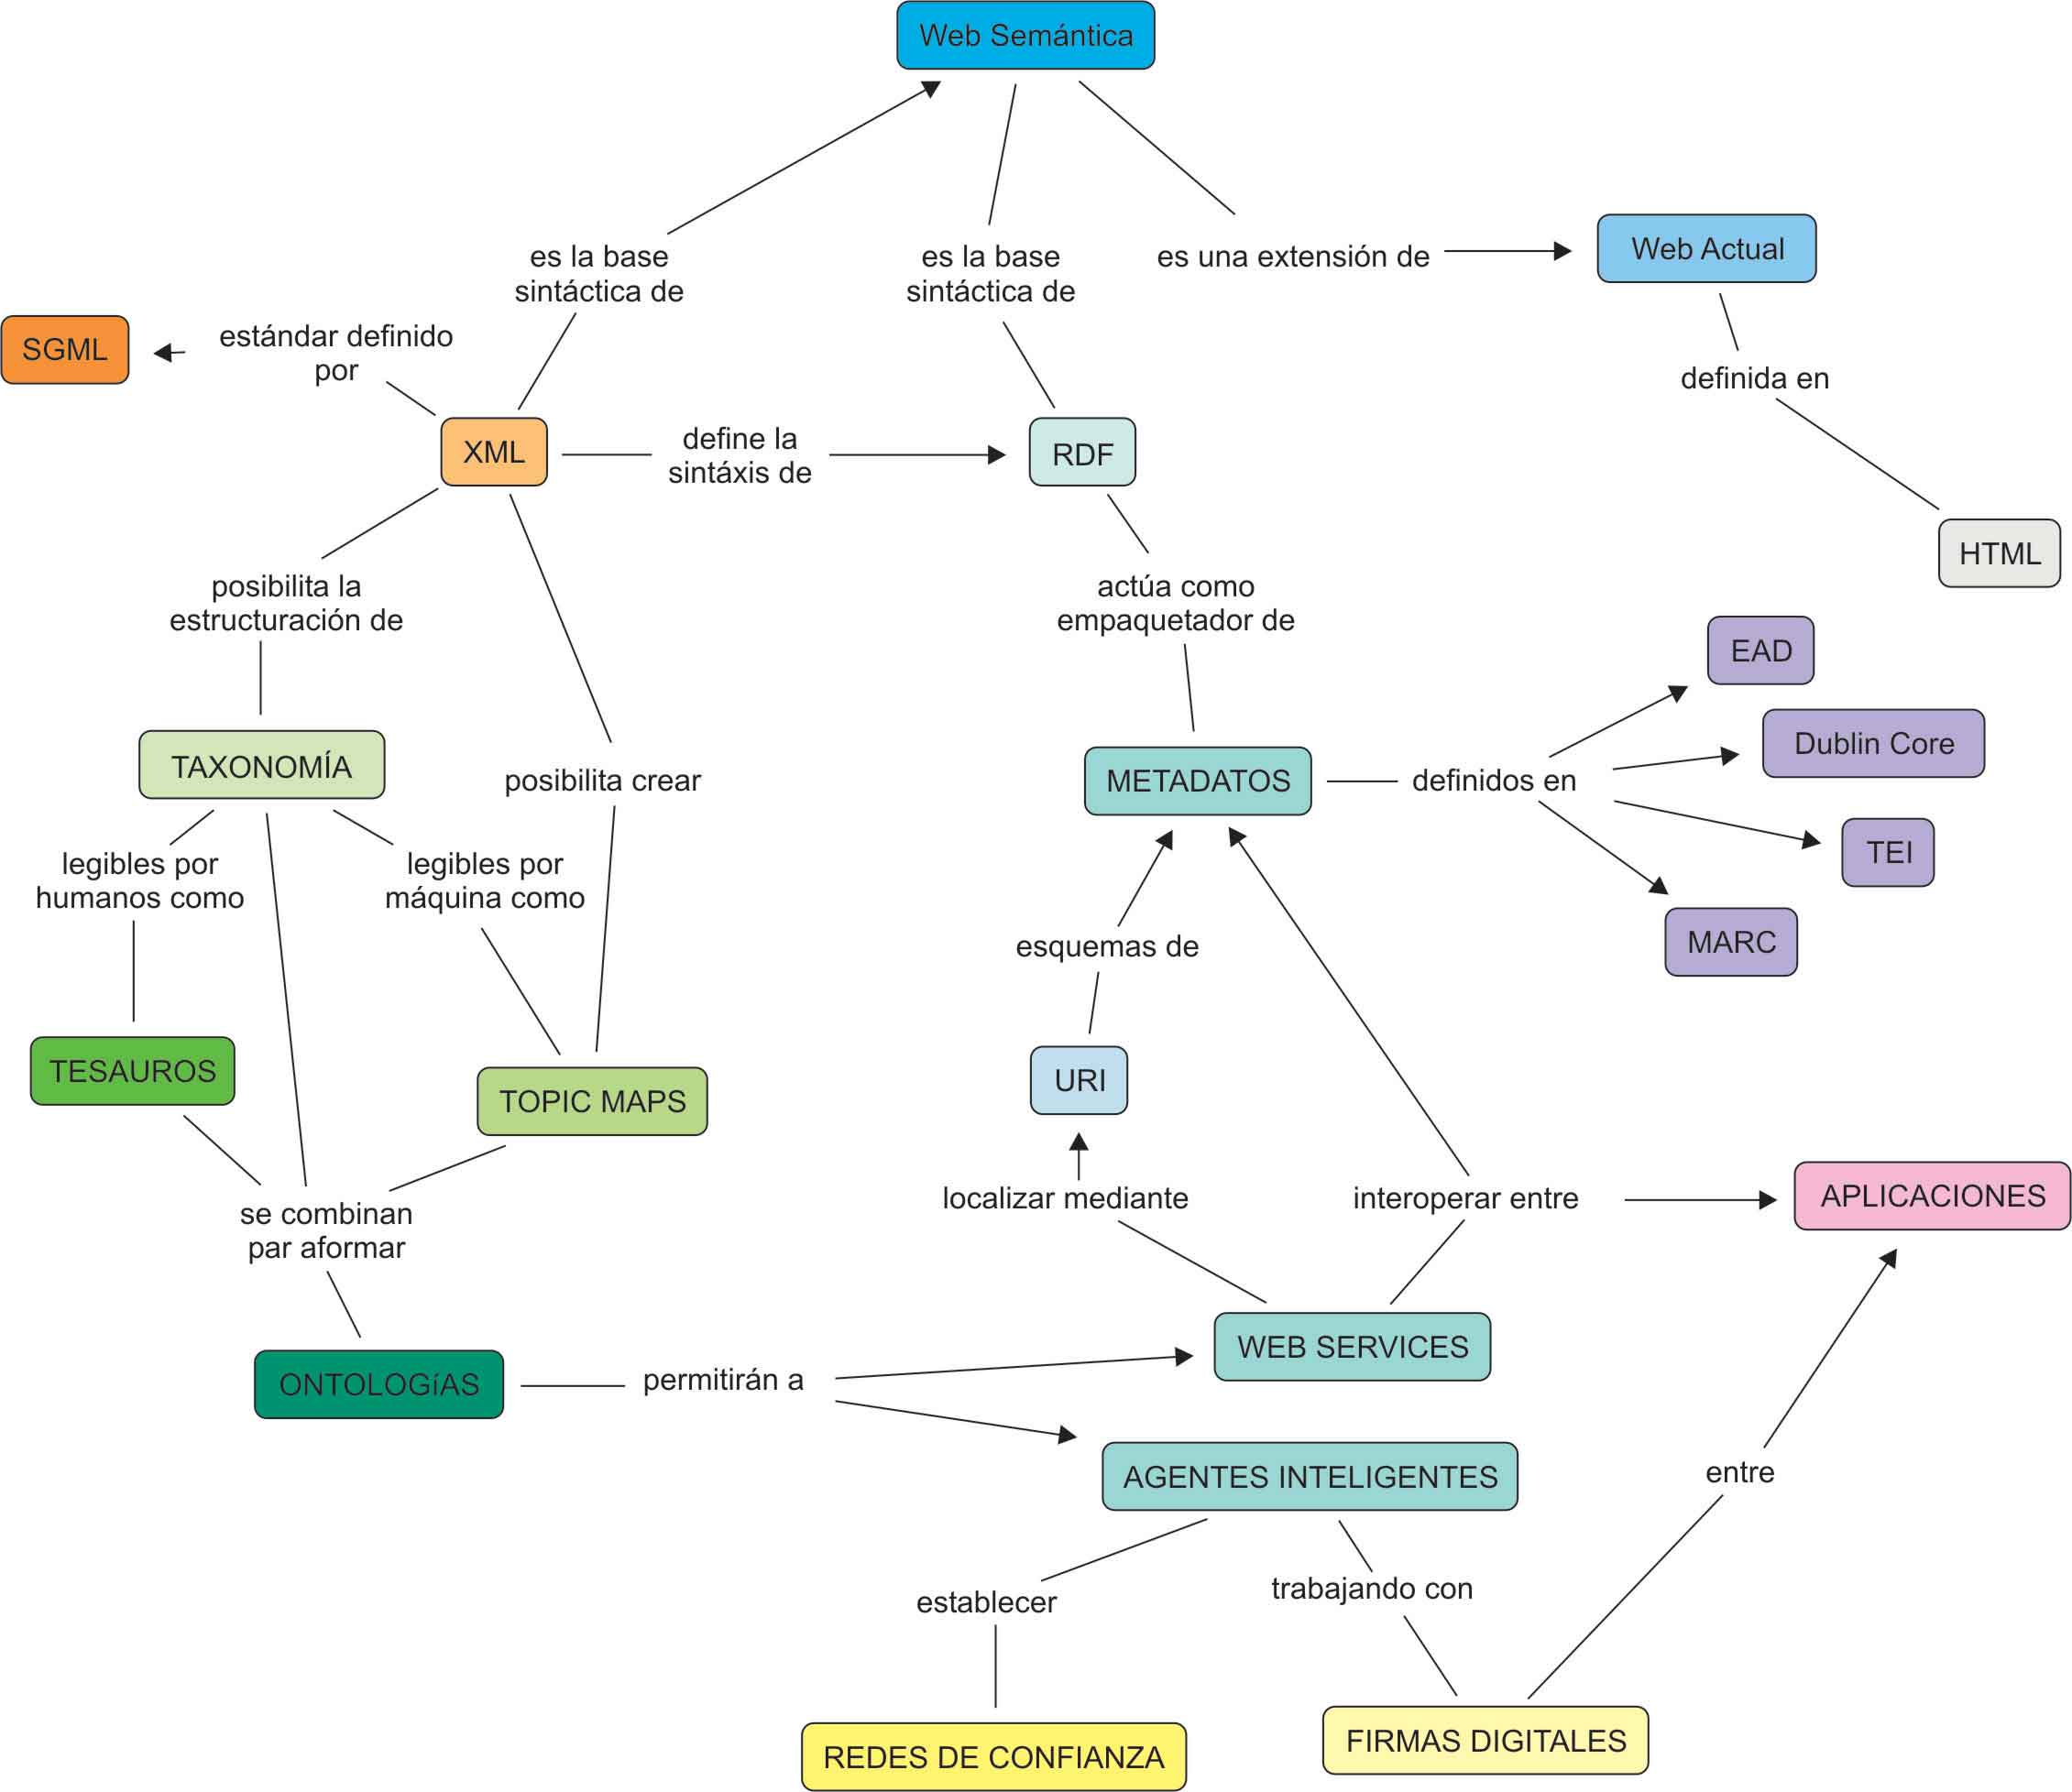
\includegraphics[width=0.9\linewidth,keepaspectratio]{ont2.jpg}
\end{center}

Ontología Cruzar - http://idi.fundacionctic.org/cruzar/turismo.owl\\
Fundación CTIC\\
Ontología de dominio. Captura la semántica de tres tipos de entidades: recursos turísticos de la ciudad de Zaragoza, perfiles de usuario y rutas turísticas, describiendo las características de una visita turística. Contiene 14 términos.

\begin{center}
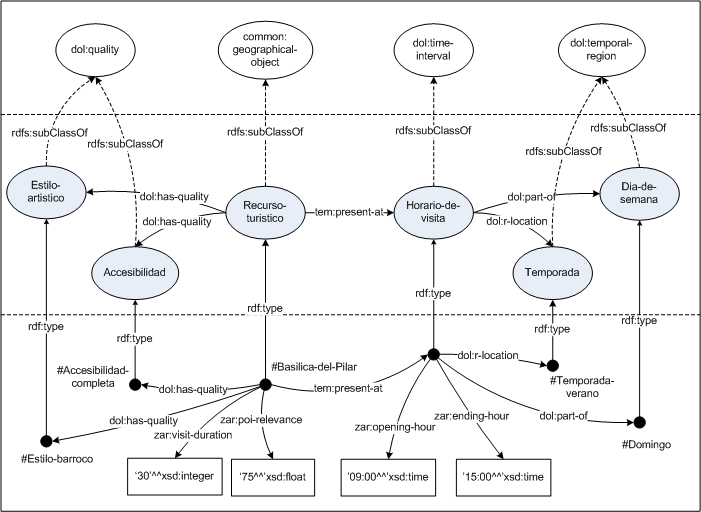
\includegraphics[width=0.9\linewidth,keepaspectratio]{ont3.png}
\end{center}

Mantis - http://www.yumpu.com/es/document/view/19123696/departamento-de-informatica-universidad-de-castilla-la-mancha-/5\\
MANTIS Software Company\\
Ontología de dominio. Gestión de proyectos de mantenimiento de sofware. Contiene aproximadamente 8 términos.

\begin{center}
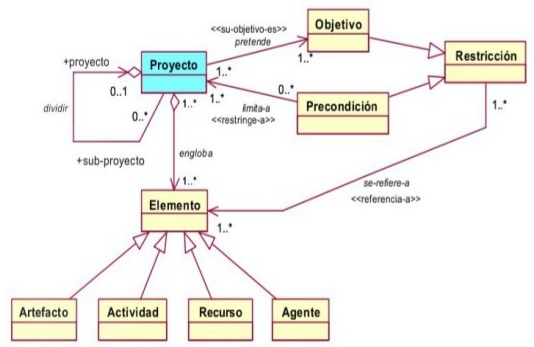
\includegraphics[width=0.7\linewidth,keepaspectratio]{ont4.jpg}
\end{center}

\end{quote}

\section*{Ejercicio 2}

¿Qué es una ontología lingüística? Explique y ejemplifique. 

\dotfill

Se vinculan a aspectos lingüísticos, esto es, a aspectos gramáticos, semánticos y sintácticos destinados a su utilización por los seres humanos.\\
Por ejemplo, en el caso de la creación de metadatos Dublin Core, se tenías metadatos destinados a ser interpretados por las personas en el archivo html.

\section*{Ejercicio 3}

Según lo expresado por Oscar Corcho en su artículo “Ontology  based 
document annotation: trends and open research problems”, responda: 

\begin{enumerate}[a.]
\item  En los que respecta a las ontologías Dublín Core y FOAF (Friend 
of a Friend):
\begin{enumerate}[I.]
\item ¿Cuál es el dominio de aplicación?

\dotfill

\begin{quote}
El dominio de Dublin Core son los documentos electrónicos. El dominio de FOAF son las web vinculadas con páginas para personas, grupos, empresas, etc.
\end{quote}

\item ¿En qué lenguaje están implementadas?

\dotfill

\begin{quote}
Dublin Core se encuentra implementada en RDF y XML. FOAF se encuentra implementada en RDF Schema.
\end{quote}

\item ¿En qué lugar se encuentran dentro de la progresión semántica propuesta por Lassila y Mc Guinness (2001)? Justifique.

\dotfill

\begin{quote}
Se encuentran de lado izquierdo puesto que poseen conceptos, taxonomías de conceptos, relaciones entre conceptos y propiedades que describen relaciones pero no modelan el dominio de manera más profunda ni agregan axiomas y restricciones.
\end{quote}

\end{enumerate}
\item Explique las relaciones y diferencias semánticas entre diferentes anotaciones: Dublín Core – Tesauro sobre información geográfica (Getty Thesaurus of Geographic Names) – Ontología en el dominio de los viajes. Ejemplifique.

\dotfill

\begin{quote}
En el caso de Dublin Core se pueden apreciar las etiquetas que responden al pedido del vuelo, quién lo realizo, fecha, descripción, etc. Para el caso del tesauro se establecen relaciones entre términos que se vinculan hasta llegar a una conclusión. El primer caso es mucho más simple de entender para la persona mientras que el tesauro contiene ciertos aspectos que lo hacen más difícil de interpretar.
\end{quote}

\item ¿Para qué se utilizan las recomendaciones de W3C, RDF, RDF Schema y OWL? Cómo se utilizan? Indique brevemente.

\dotfill

\begin{quote}
Se utilizan para implementar las ontologías y sus anotaciones. Se utilizan insertando en el código correspondiente a una de las recomendaciones en el código HTML de la página web o dentro de cualquier otro recurso web.
\end{quote}

\item ¿Qué son las herramientas para anotación de metadatos basadas en ontologías?\\
Seleccione una herramienta. Describa su funcionamiento. Ejemplifique.  

\dotfill

\begin{quote}
Son diseñadas principalmente para permitir la inserción y el mantenimiento de anotaciones basadas en ontologías en páginas Web.\\

\textit{OntoMat-Annotizer}\\
Esta herramienta permite arrastrar y soltar partes del texto en las anotaciones que se están creando. Con esta herramienta, los usuarios pueden crear instancias de sus atributos y instancias de relación. En la parte izquierda de la interfaz de usuario, podemos ver atributos y relaciones de la instancia seleccionada que puede ser completado. En el caso de las relaciones, la herramienta también presenta las instancias que pueden estar relacionadas con la instancia seleccionada con esa relación. OntoMat-Annotizer carga ontologías OWL. Las anotaciones creadas con esta herramienta se almacenan en OWL, ya sea como archivos o incrustados en los documentos HTML anotados. Estas anotaciones pueden ser utilizadas por una amplia gama de aplicaciones en la web semántica.
\end{quote}

\end{enumerate}

\begin{thebibliography}{1} 
\bibitem{ONTO}
Oscar Corcho,
\emph{Artículo - Ontology based document annotation: trends and open research problems},
Int. J. Metadata, Semantics and Ontologies, Vol. 1, N 1, 
2006.

\bibitem{SWP}
Grigoris Antoniou and Frank van Harmelen,
\emph{A Semantic Web Primer. Second edition},
Massachusetts Institute of Technology,
2008.

\bibitem{DW}
\emph{Acceso  a  documentos  Web  para  búsqueda  y 
selección de información}.
\end{thebibliography}

\end{document}